
\documentclass[a4paper,12pt]{scrbook}
\usepackage{amsmath,amssymb,amsthm}
\usepackage{fancyvrb}
\usepackage{parskip}
\usepackage{lastpage}
\usepackage{verbatim,boxedminipage,enumitem}
\usepackage{ifthen}
\usepackage{color,graphicx}
\usepackage{pgf}
\usepackage{longtable}
\usepackage{upquote}
%\usepackage[all]{xy}
\usepackage{tobiShell}
\usepackage{tikz}
\usetikzlibrary{automata}
\usetikzlibrary{arrows}
\usepackage{pgf,pgfarrows,pgfnodes}
\usepackage{pgfplots}
\usepackage{circuitikz}
\usetikzlibrary{circuits}
\usetikzlibrary{circuits.logic.US}
\usepackage{mymath}
\usepackage{python}
%------------------------------------------------------------------
% Verbatim for console window - single line frame, no line numbers
%------------------------------------------------------------------
\DefineVerbatimEnvironment%
 {console}{Verbatim}
 {frame=single}

%--------------------------------------------------------
% Remove the vertical spacing before and after Verbatim.
%--------------------------------------------------------
\usepackage{atbeginend}
\BeforeBegin{console}{\mbox{}\\ \begin{minipage}{\textwidth}\vspace{3pt}}
\AfterEnd{console}{\vspace{4pt} \end{minipage} \\ }

\begin{document}
\thispagestyle{empty}

\begin{center}
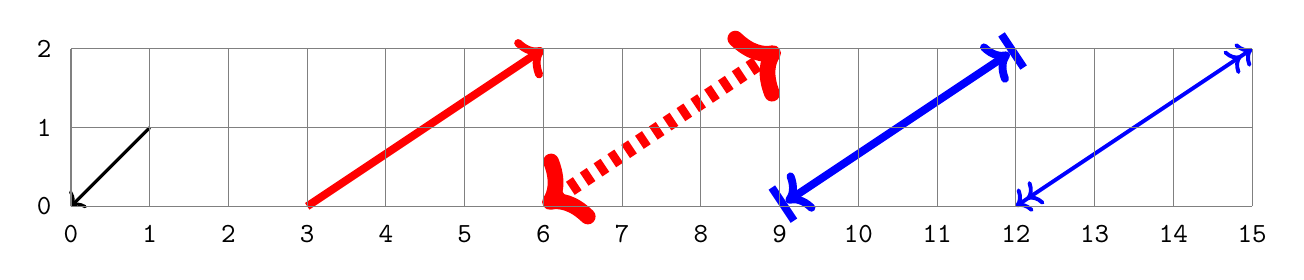
\begin{tikzpicture}
\draw[line width=0.04cm,black,<-] (0.0,0.0) -- (1.0,1.0);
\draw[line width=0.1cm,red,->] (3.0,0.0) -- (6.0,2.0);
\draw[line width=0.2cm,red,<->,dashed] (6.0,0.0) -- (9.0,2.0);
\draw[line width=0.1cm,blue,|<->|] (9.0,0.0) -- (12.0,2.0);
\draw[line width=0.05cm,blue,<<->>] (12.0,0.0) -- (15.0,2.0);
\draw[gray] (0.0,0.0) -- (0.0,2);
\draw[gray] (1.0,0.0) -- (1.0,2);
\draw[gray] (2.0,0.0) -- (2.0,2);
\draw[gray] (3.0,0.0) -- (3.0,2);
\draw[gray] (4.0,0.0) -- (4.0,2);
\draw[gray] (5.0,0.0) -- (5.0,2);
\draw[gray] (6.0,0.0) -- (6.0,2);
\draw[gray] (7.0,0.0) -- (7.0,2);
\draw[gray] (8.0,0.0) -- (8.0,2);
\draw[gray] (9.0,0.0) -- (9.0,2);
\draw[gray] (10.0,0.0) -- (10.0,2);
\draw[gray] (11.0,0.0) -- (11.0,2);
\draw[gray] (12.0,0.0) -- (12.0,2);
\draw[gray] (13.0,0.0) -- (13.0,2);
\draw[gray] (14.0,0.0) -- (14.0,2);
\draw[gray] (15.0,0.0) -- (15.0,2);
\draw[gray] (0.0,0.0) -- (15,0.0);
\draw[gray] (0.0,1.0) -- (15,1.0);
\draw[gray] (0.0,2.0) -- (15,2.0);
\draw(0, 0) node [font=\ttfamily, label=below:{\texttt{0}}] {};
\draw(1, 0) node [font=\ttfamily, label=below:{\texttt{1}}] {};
\draw(2, 0) node [font=\ttfamily, label=below:{\texttt{2}}] {};
\draw(3, 0) node [font=\ttfamily, label=below:{\texttt{3}}] {};
\draw(4, 0) node [font=\ttfamily, label=below:{\texttt{4}}] {};
\draw(5, 0) node [font=\ttfamily, label=below:{\texttt{5}}] {};
\draw(6, 0) node [font=\ttfamily, label=below:{\texttt{6}}] {};
\draw(7, 0) node [font=\ttfamily, label=below:{\texttt{7}}] {};
\draw(8, 0) node [font=\ttfamily, label=below:{\texttt{8}}] {};
\draw(9, 0) node [font=\ttfamily, label=below:{\texttt{9}}] {};
\draw(10, 0) node [font=\ttfamily, label=below:{\texttt{10}}] {};
\draw(11, 0) node [font=\ttfamily, label=below:{\texttt{11}}] {};
\draw(12, 0) node [font=\ttfamily, label=below:{\texttt{12}}] {};
\draw(13, 0) node [font=\ttfamily, label=below:{\texttt{13}}] {};
\draw(14, 0) node [font=\ttfamily, label=below:{\texttt{14}}] {};
\draw(15, 0) node [font=\ttfamily, label=below:{\texttt{15}}] {};
\draw(0, 0) node [font=\ttfamily, label=left:{\texttt{0}}] {};
\draw(0, 1) node [font=\ttfamily, label=left:{\texttt{1}}] {};
\draw(0, 2) node [font=\ttfamily, label=left:{\texttt{2}}] {};
\end{tikzpicture}

\end{center}

\end{document}
